\section{Question 1}

Given:
\[
w_1=\begin{cases}
1&\text{Prob }1/2\\
3&\text{Prob }1/2
\end{cases}
\qquad
c(x)=\begin{cases}
x&\text{if }x\ge0\\
-1000x&\text{if }x<0
\end{cases}
\]
\[
g_t(x_t,u_t)=c(x_t)+2u_t,\qquad g_N(x_N)=c(x_N)
\]

let's start DP with terminal cost

at $t=N=2$
\[
g_2(x_2)=c(x_2)=
\begin{cases}
x_2&x_2\ge0\\
-1000x_2&x_2<0
\end{cases}
\qquad J_2^*(x_2)=g_2(x_2)
\]

at $t=N-1$

using DP
\begin{align*}
J_1^*(x_1)&=\E_{w_1}\left[c(x_1)+2u_1+J_2^*(x_2)\mid x_1,u_1\right]\\
&=c(x_1)+2u_1+\E_{w_1}\left[J_2^*(x_1+u_1-w_1)\right]\\
&=c(x_1)+2u_1+\frac12J_2^*(x_1+u_1-1)+\frac12J_2^*(x_1+u_1-3)
\end{align*}

let
\[
F(u_1)=\begin{cases}
2u_1+\frac12[-1000(x_1+u_1-1)]+\frac12[-1000(x_1+u_1-3)]
&x_1+u_1<1\\[2mm]
2u_1+\frac12(x_1+u_1-1)+\frac12[-1000(x_1+u_1-3)]
&1\le x_1+u_1<3\\[2mm]
2u_1+\frac12(x_1+u_1-1)+\frac12(x_1+u_1-3)
&x_1+u_1\ge3
\end{cases}
\]
\[
F(u_1)=\begin{cases}
-998u_1-1000x_1+2000&u_1<1-x_1\\[1mm]
-\dfrac{995u_1}{2}-\dfrac{999x_1}{2}+\dfrac{2999}{2}
&1-x_1\le u_1<3-x_1\\[2mm]
3u_1+x_1-2&u_1\ge3-x_1
\end{cases}
\]
\begin{center}
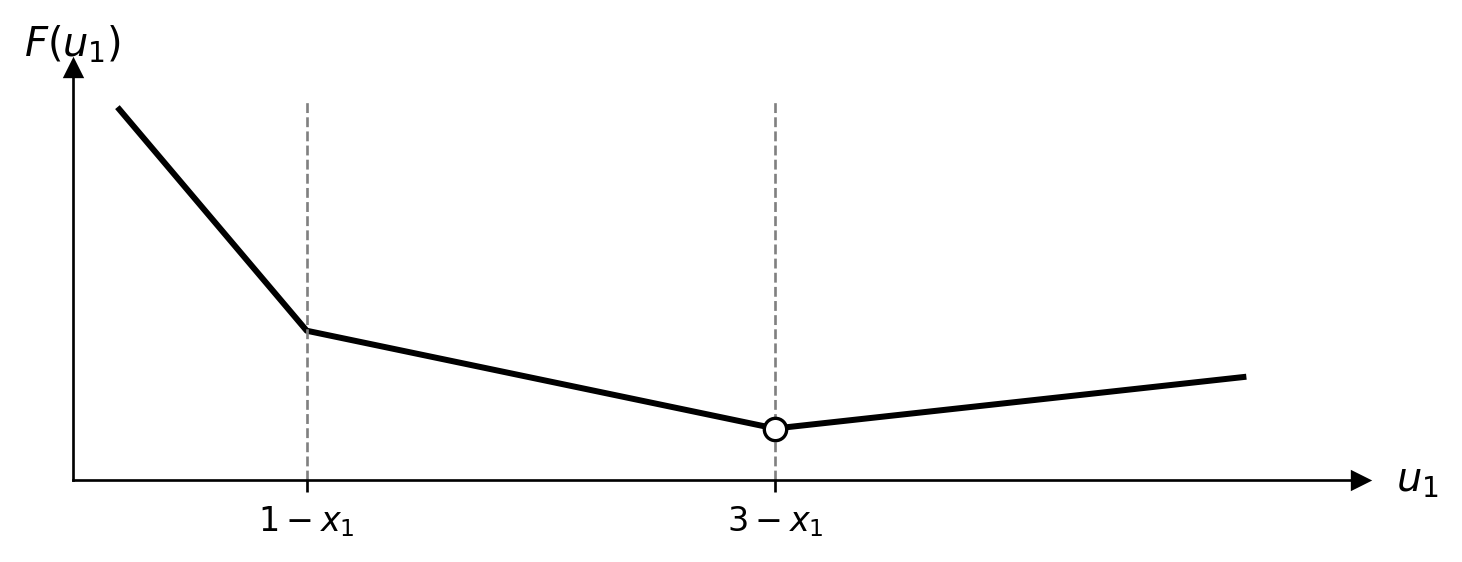
\includegraphics[width=0.60\textwidth,height=1.45in,keepaspectratio]{report_figures/q1_stage1.png}
\end{center}
\[
F(u_1)=\text{minimum at }u_1^*=3-x_1
\]
\[
\boxed{J_1^*(x_1)=c(x_1)+7-2x_1\quad\text{at }u_1^*=3-x_1}
\]

\clearpage
now
\begin{align*}
J_0(x_0)&=\E_{w_0}\left[c(x_0)+2u_0+J_1^*(x_1)\mid x_0,u_0\right]\\
&=c(x_0)+2u_0+\E_{w_0}\left[J_1^*(x_0+u_0-w_0)\right]\\
&=c(x_0)+\underbrace{2u_0+\frac12J_1^*(x_0+u_0-1)
+\frac12J_1^*(x_0+u_0-3)}_{F(u_0)}
\end{align*}
\[
J_1^*(x_1)=\begin{cases}
-1000x_1+7-2x_1&x_1<0\\
7-x_1&x_1\ge0
\end{cases}
\]
\[
F(u_0)=\begin{cases}
2u_0+\dfrac{-1002(x_0+u_0-1)+7}{2}
+\dfrac{-1002(x_0+u_0-3)+7}{2}
&x_0+u_0<1\\[3mm]
2u_0+\dfrac{7-(x_0+u_0-1)}{2}
+\dfrac{-1002(x_0+u_0-3)+7}{2}
&1\le x_0+u_0<3\\[3mm]
2u_0+\dfrac{7-(x_0+u_0-1)}{2}
+\dfrac{7-(x_0+u_0-3)}{2}
&x_0+u_0\ge3
\end{cases}
\]
\[
F(u_0)=\begin{cases}
-1000u_0-1002x_0+2011&u_0<1-x_0\\[1mm]
-\dfrac{999u_0}{2}-\dfrac{1003x_0}{2}+\dfrac{3021}{2}
&1-x_0\le u_0<3-x_0\\[2mm]
u_0-x_0+9&u_0\ge3-x_0
\end{cases}
\]
\begin{center}
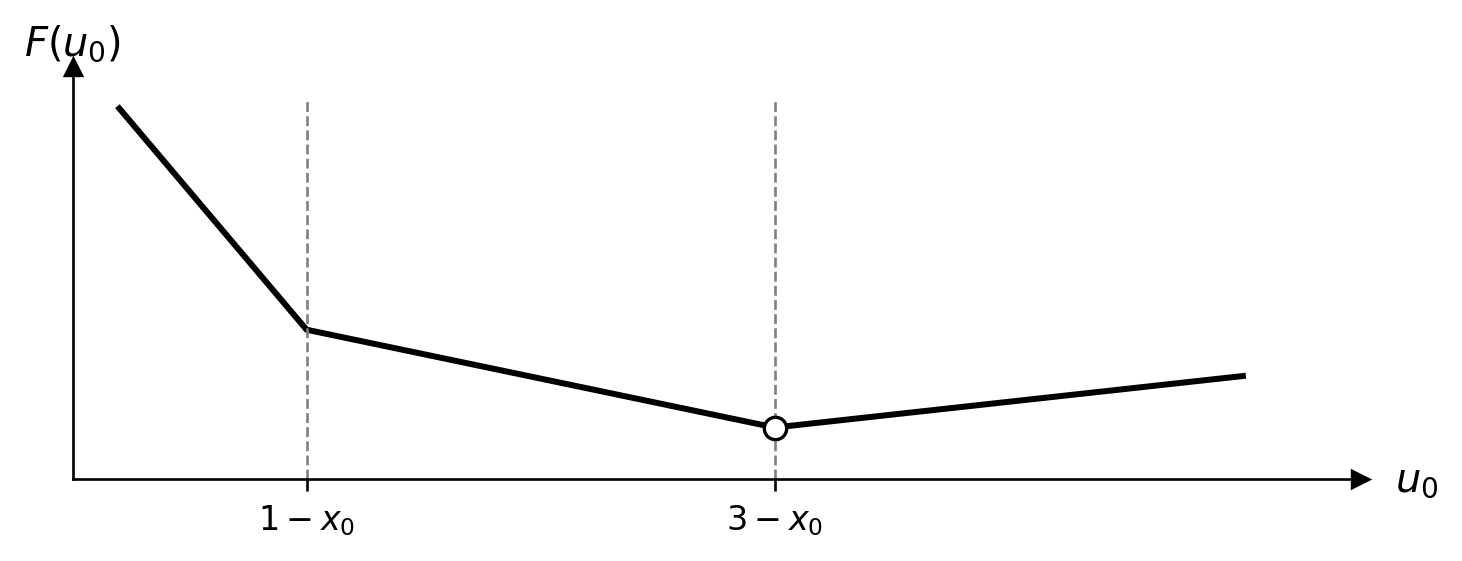
\includegraphics[width=0.75\textwidth,height=2.05in,keepaspectratio]{report_figures/q1_stage0.png}
\end{center}

optimum value occurs at
\[
u_0^*=3-x_0
\]
\[
F(u_0^*)=12-2x_0
\]
\[
\boxed{J_0^*(x_0)=c(x_0)+12-2x_0}
\]
\[
J_0^*(0)=12
\]
